\subsection{Dobozmodell}

%30
\begin{frame}
  \begin{columns}[c]
    \column{0.5\textwidth}
      Minden HTML elemet egy \emph{doboznak} tekintünk. Ezek szerkezete belülről kifelé:
      \begin{itemize}
        \item Az elem tartalma (szöveg, kép, \dots)
        \item Kitöltés (\texttt{padding}; átlátszó)
        \item Szegély (\texttt{border})
        \item Margó (\texttt{margin}; átlátszó)
      \end{itemize}
      \vfill
      Megjegyzések
      \begin{itemize}
        \item A szélesség (\texttt{width}) és magasság (\texttt{height}) 
      tulajdonságok a tartalmi rész méreteire vonatkoznak.
        \item Soron belüli elemek méretét a böngésző határozza 
        meg, nem méretezhetőek át.
      \end{itemize}
    \column{0.5\textwidth}
      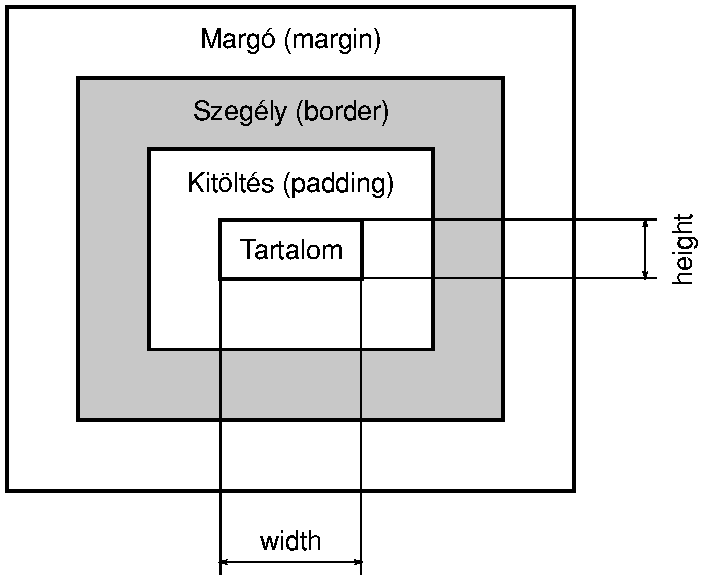
\includegraphics[width=\textwidth]{doboz.pdf}
  \end{columns} 
\end{frame}

%31
\begin{frame}
  \begin{columns}[c]
    \column{0.45\textwidth}
      \begin{exampleblock}{\textattachfile{dobozMeret.html}{dobozMeret.html}}
        \tiny
        \lstinputlisting[style=HTML,linerange={7-18},numbers=left,firstnumber=7]{dobozMeret.html}
      \end{exampleblock}
    \column{0.55\textwidth}
      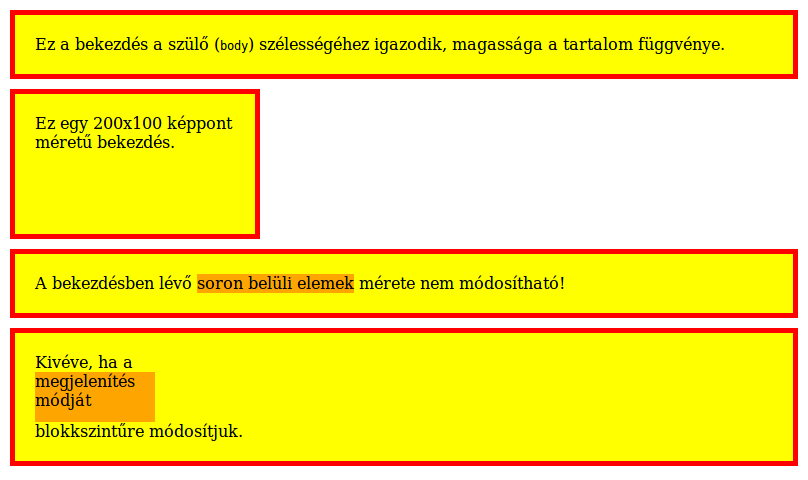
\includegraphics[width=0.9\textwidth]{dobozMeret.png}
  \end{columns}
  \begin{exampleblock}{\vspace*{-3ex}}
    \tiny
    \lstinputlisting[style=HTML,linerange={22-25},numbers=left,firstnumber=22]{dobozMeret.html}
  \end{exampleblock}
\end{frame}

%32
\begin{frame}
\begin{columns}[c]
  \column{0.5\textwidth}
    Mit számol bele a böngésző a méret (\texttt{width}, 
    \texttt{height}) adatokba? $\to$ \texttt{box-sizing}
    \begin{description}[m]
      \item[\texttt{content-box}] \hfill \\ 
        Csak a tartalom méretét
      \item[\texttt{border-box}] \hfill \\ 
        Tartalom + kitöltés + szegély
    \end{description}
    \vfill
    Kényelmes:\\
    \texttt{* \{ box-sizing: border-box; \} }
  \column{0.5\textwidth}
    \begin{center}
      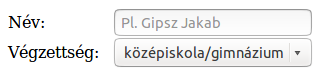
\includegraphics[scale=0.5]{meretezes.png}
    \end{center}
    \begin{exampleblock}{\textattachfile{meretezes.html}{meretezes.html}}
      \scriptsize
      \lstinputlisting[style=HTML,linerange={11-17},numbers=left,firstnumber=11]{meretezes.html}
    \end{exampleblock}
\end{columns} 
  
\end{frame}
